\coverchapter{Results}\label{ch:results}

The search method we have developed and the resulting bijections work between different domains. The problem, however, is the lack of existing implementations of domains using Combinatorial Exploration. With Combinatorial Exploration being a product of a research group that is mainly interested in permutation patterns, unsurprisingly, the most supported domain is permutations with \tsc{}. As a consequence, we will mostly demonstrate bijections found between permutation classes.

\section{Cross-domain successes}
There is a simple example implementation of words provided in the repository for Combinatorial Exploration. A word over an alphabet $\Sigma$ is any sequence of elements from $\Sigma$. A pattern in a word is another word that occurs as a consecutive subsequence. A class can be described as a triple $\mathcal{W} = (p, \Sigma, A)$, where $p$ is a required prefix, $\Sigma$ is the alphabet and $A$ is the set of patterns to avoid. For example $(\varepsilon, \set{0,1}, \set{11})$ is the set of binary strings that avoid consecutive 1's, that is
\[
    (\varepsilon, \set{0,1}, \set{11}) = \set{\varepsilon, 0, 1, 00, 01, 10, 000, 001, 010, 100, 101, \dotsc}.
\]


The bijection search will easily find bijections between sets such as $(\varepsilon, \set{0,1}, \set{11})$ and $(\varepsilon, \set{a,b}, \set{bb})$, that are identical given a bijection of the letters of the alphabet. The same goes for the trivial sets $(\epsilon, \set{0}, \emptyset)$ and $\Av{12}$, where there is only a single element of each size. The implementation for words has few strategies and limited effort was allocated to finding bijections between words and permutation classes. We will demonstrate two such bijections in greater detail but there is a caveat that needs to be addressed.

Consider the class $\mathcal{W} = (\varepsilon, \set{a,b}, \emptyset)$. For any fixed size $n$, there are $2^n$ unique words as we have a choice between two letters for each position in any sequence. This produces the counting sequence $1, 2, 4, 8, 16, 32, 64, \dotsc$ while the permutation class we want to match with, $\Av{231,321}$, has the counting sequence $1, 1, 2, 4, 8, 16, 32, \dotsc$ which is off by one. We could use $\textsf{Av}_{\geq1}(231,312)$ instead, which shares this sequence with the words if we start from $n=1$, but that brings another problem. Words of size $n$ would map to permutations of size $n+1$ while parallel specifications require atoms to match. What we can do instead is place the topmost point of $\textsf{Av}_{\geq1}(231,312)$ and factor it out. That leaves us with a tiling root $\mathcal{T}$ where
\begin{align*}
    \Av{231,312} &\cong \set{\varepsilon} \sqcup \textsf{Av}_{\geq1}(231,312),\\
    \textsf{Av}_{\geq1}(231,312) &\cong \set{\point{0.1}}\times \textsf{Grid}(\mathcal{T}).
\end{align*}
The tiling in question here is
\[
    \mathcal{T} = \left((2,1), \set{2^{(0,0)}1^{(1,0)}, 21^{(1,0)}, 231^{(0,0)}, 321^{(0,0)}},\emptyset\right),
\]
shown in \FigureRef{fig:wordtiling}.
\begin{figure}[ht!]
    \centering
    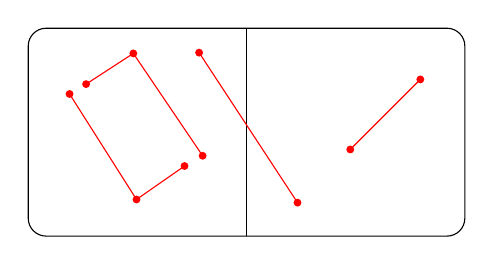
\begin{tikzpicture}[scale=0.5, every node/.style={scale=0.5}]
        \def\xscale{1.0} % Horizontal scale factor
        \def\yscale{1.0} % Vertical scale factor
        \def\spnt{0.1} % Size of smaller points
        \def\lpnt{0.125} % Size of larger points
        \def\roundscale{0.75} % The rounding factor
        \draw[rounded corners=2ex*\roundscale] (0,0) rectangle (11.09*\xscale,5.28*\yscale);
        \draw (5.545*\xscale, 5.28*\yscale) -- (5.545*\xscale, 0);
        \fill[red] (8.18*\xscale, 2.2*\yscale) circle (\spnt);
        \fill[red] (9.96*\xscale, 3.98*\yscale) circle (\spnt);
        \draw[red] (8.18*\xscale, 2.2*\yscale) -- (9.96*\xscale,3.98*\yscale);
        \fill[red] (4.34*\xscale, 4.66*\yscale) circle (\spnt);
        \fill[red] (6.84*\xscale, 0.85*\yscale) circle (\spnt);
        \draw[red] (4.34*\xscale, 4.66*\yscale) -- (6.84*\xscale,0.85*\yscale);
        \fill[red] (1.47*\xscale, 3.86*\yscale) circle (\spnt);
        \fill[red] (2.67*\xscale, 4.64*\yscale) circle (\spnt);
        \fill[red] (4.43*\xscale, 2.04*\yscale) circle (\spnt);
        \draw[red] (1.47*\xscale, 3.86*\yscale) -- (2.67*\xscale,4.64*\yscale) -- (4.43*\xscale,2.04*\yscale);
        \fill[red] (1.05*\xscale, 3.61*\yscale) circle (\spnt);
        \fill[red] (2.75*\xscale, 0.93*\yscale) circle (\spnt);
        \fill[red] (3.97*\xscale, 1.78*\yscale) circle (\spnt);
        \draw[red] (1.05*\xscale, 3.61*\yscale) -- (2.75*\xscale,0.93*\yscale) -- (3.97*\xscale,1.78*\yscale);
\end{tikzpicture}
    \caption{The tiling used instead of $\Av{231,312}$ to deal with the sequence offset of binary strings.}
    \label{fig:wordtiling}
\end{figure}
Now we can find and construct bijections between $\mathcal{W}$ and $\textsf{Grid}(\mathcal{T})$. It will map the words to gridded permutations in $\mathcal{G}^{(2,1)}$ instead of $\mathcal{G}^{(1,1)}$ but there is a trivial bijection from these gridded permutations to permutations in $\textsf{Av}_{\geq1}(231,312)$.

The other bijection found was between $\mathcal{W} = (\varepsilon, \set{0,1}, \set{11})$ and $\Av{231,312,321}$. These are counted by the Fibonacci numbers but here we have the same issue as before, with one sequence being off by one. We remedy this in the same way as before, leaving us with a tiling root that can be seen in \FigureRef{fig:fibpermoffbyone}. This tiling can have at most a single point in cell $(1,0)$ and if it includes one, it must be greater than all the points in cell $(0,0)$. We can map any such gridded permutation to a permutation with a trivial bijection. Given a gridded permutation of size $n$ that contains no point in cell $(1,0)$ we append $n+1$ to the underlying permutation. If it contains a point in $(1,0)$ we place $n+1$ immediately prior to the last element.

\begin{figure}[!htbp]
    \centering
    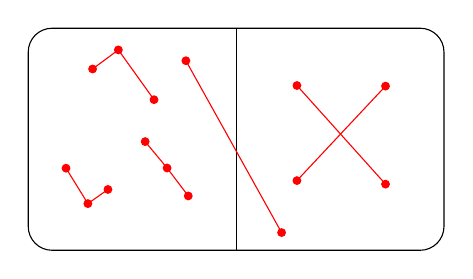
\begin{tikzpicture}[scale=1, every node/.style={scale=1}]
    \def\xscale{0.75} % Horizontal scale factor
    \def\yscale{0.75} % Vertical scale factor
    \def\spnt{0.075*0.75} % Size of smaller points
    \def\lpnt{0.125*0.75} % Size of larger points
    \draw (3.52*\xscale, 3.76*\yscale) -- (3.52*\xscale, 0);
    \draw[rounded corners=2ex] (0,0) rectangle (7.04*\xscale,3.76*\yscale);
    
    \fill[red] (4.55*\xscale, 1.18*\yscale) circle (\spnt);
    \fill[red] (6.05*\xscale, 2.78*\yscale) circle (\spnt);
    \draw[red] (4.55*\xscale, 1.18*\yscale) -- (6.05*\xscale,2.78*\yscale);
    
    \fill[red] (4.55*\xscale, 2.79*\yscale) circle (\spnt);
    \fill[red] (6.05*\xscale, 1.12*\yscale) circle (\spnt);
    \draw[red] (4.55*\xscale, 2.79*\yscale) -- (6.05*\xscale,1.12*\yscale);
    
    \fill[red] (2.67*\xscale, 3.21*\yscale) circle (\spnt);
    \fill[red] (4.29*\xscale, 0.3*\yscale) circle (\spnt);
    \draw[red] (2.67*\xscale, 3.21*\yscale) -- (4.29*\xscale,0.3*\yscale);
    
    \fill[red] (1.09*\xscale, 3.07*\yscale) circle (\spnt);
    \fill[red] (1.526001050877835*\xscale, 3.393088634545991*\yscale) circle (\spnt);
    \fill[red] (2.13*\xscale, 2.55*\yscale) circle (\spnt);
    \draw[red] (1.09*\xscale, 3.07*\yscale) -- (1.526001050877835*\xscale,3.393088634545991*\yscale) -- (2.13*\xscale,2.55*\yscale);
    
    \fill[red] (0.64*\xscale, 1.39*\yscale) circle (\spnt);
    \fill[red] (1.01*\xscale, 0.79*\yscale) circle (\spnt);
    \fill[red] (1.35*\xscale, 1.03*\yscale) circle (\spnt);
    \draw[red] (0.64*\xscale, 1.39*\yscale) -- (1.01*\xscale,0.79*\yscale) -- (1.35*\xscale,1.03*\yscale);
    
    \fill[red] (1.98*\xscale, 1.84*\yscale) circle (\spnt);
    \fill[red] (2.3511520552717013*\xscale, 1.3932029657051672*\yscale) circle (\spnt);
    \fill[red] (2.71*\xscale, 0.92*\yscale) circle (\spnt);
    \draw[red] (1.98*\xscale, 1.84*\yscale) -- (2.3511520552717013*\xscale,1.3932029657051672*\yscale) -- (2.71*\xscale,0.92*\yscale);
\end{tikzpicture}
    \caption{The tiling used instead of $\Av{231,312,321}$ to deal with the sequence offset of binary strings with no consecutive 1's.}
    \label{fig:fibpermoffbyone}
\end{figure}

\FigureRef{fig:fibwordtree} and \FigureRef{fig:fibpermtree} show the two parallel specifications that were found. Note that there is an empty class in the specification for words. \TableRef{tab:wordtilmap} shows the inputs and outputs up to size $3$ for the bijection constructed and corresponding permutation with the mapping described above. 

\begin{table}[ht!]
    \centering
    \begin{tabular}{c|c|c}
    Word & Gridded permutation & Permutation\\
    \hline
    $\varepsilon$ & $\varepsilon$ & $1$\\
    $0$ & $1^{(0,0)}$ & $12$\\
    $1$ & $1^{(1,0)}$ & $21$\\
    $00$ & $12^{(0,0)}$ & $123$\\
    $01$ & $21^{(0,0)}$ & $213$\\
    $10$ & $1^{(0,0)}2^{(1,0)}$ & $132$\\
    $000$ & $123^{(0,0)}$ & $1234$\\
    $001$ & $213^{(0,0)}$ & $2134$\\
    $010$ & $132^{(0,0)}$ & $1324$\\
    $100$ & $12^{(0,0)}3^{(1,0)}$ & $1243$\\
    $101$ & $21^{(0,0)}3^{(1,0)}$ & $2143$\\
\end{tabular}
    \caption{The inputs and outputs up to size $3$ of an automated bijection between binary strings avoiding consecutive 1's and $\textsf{Grid}(\mathcal{T})$, where $\mathcal{T}$ is the tiling for $\textsf{Av}_{\geq1}(231,312,321)$ after placing and factoring out the top point. The corresponding permutation is also shown.}
    \label{tab:wordtilmap}
\end{table}

\begin{figure}
    \centering
    % TODO: Redo this crap properly 

{
\newcommand{\wordclass}[2]{%
\begin{tikzpicture}[scale=0.3, baseline=(current bounding box.center)]
\useasboundingbox (0,-3) rectangle (#1,3);
			\draw[thick, rounded corners=3pt] (0,0) rectangle (#1,3);
			\node at ({#1/2}, 1.5) {#2};
;
			    \end{tikzpicture}
}
    \begin{center}
    \scalebox{1}{\begin{tikzpicture}[scale=0.8, every node/.style={scale=0.8}]
        \node (root) at (0, 0) {\wordclass{8}{$(\varepsilon,\set{0,1},\set{11})$}};
        \node (lvl_1_1) at (-4, -2.25) {\wordclass{8}{$(0,\set{0,1},\set{11})$}};
        \node (lvl_1_2) at (0, -2.25) {\wordclass{8}{$\set{\varepsilon}$}};
        \node (lvl_1_3) at (4, -2.25) {\wordclass{8}{$(1,\set{0,1},\set{11})$}};
        \node (lvl_2_1) at (-6, -4.5) {\wordclass{8}{$\set{0}$}};
        \node (lvl_2_2) at (-2, -4.5) {\wordclass{8}{$(\varepsilon,\set{0,1},\set{11})$}};
        \node (lvl_2_3) at (1, -4.5) {\wordclass{8}{$\set{1}$}};
        \node (lvl_2_4) at (4, -4.5) {\wordclass{8.5}{$(10,\set{0,1},\set{11})$}};
        \node (lvl_2_5) at (7, -4.5) {\wordclass{8.5}{$(11,\set{0,1},\set{11})$}};
        \node (lvl_3_1) at (2, -6.75) {\wordclass{8}{$\set{10}$}};
        \node (lvl_3_2) at (6, -6.75) {\wordclass{8.5}{$(\varepsilon,\set{0,1},\set{11})$}};
        \node (lvl_4_1) at (0, -9) {\wordclass{8}{$\set{1}$}};
        \node (lvl_4_2) at (4, -9) {\wordclass{8}{$\set{0}$}};
        \ptedge{(root)}{(-0.5,1.2)}{(lvl_1_1)}{(-0.5,1.3)}
        \ptedge{(root)}{(-0.5,1.2)}{(lvl_1_2)}{(-0.5,1.3)}
        \ptedge{(root)}{(-0.5,1.2)}{(lvl_1_3)}{(-0.5,1.3)}
        \ptedge{(lvl_1_1)}{(-0.5,1.2)}{(lvl_2_1)}{(-0.5,1.3)}
        \ptedge{(lvl_1_1)}{(-0.5,1.2)}{(lvl_2_2)}{(-0.5,1.3)}
        \ptedge{(lvl_1_3)}{(-0.5,1.2)}{(lvl_2_3)}{(-0.5,1.3)}
        \ptedge{(lvl_1_3)}{(-0.5,1.2)}{(lvl_2_4)}{(-0.5,1.3)}
        \ptedge{(lvl_1_3)}{(-0.5,1.2)}{(lvl_2_5)}{(-0.5,1.3)}
        \ptedge{(lvl_2_4)}{(-0.5,1.2)}{(lvl_3_1)}{(-0.5,1.3)}
        \ptedge{(lvl_2_4)}{(-0.5,1.2)}{(lvl_3_2)}{(-0.5,1.3)}
        \ptedge{(lvl_3_1)}{(-0.5,1.2)}{(lvl_4_1)}{(-0.5,1.3)}
        \ptedge{(lvl_3_1)}{(-0.5,1.2)}{(lvl_4_2)}{(-0.5,1.3)}
    \end{tikzpicture}}
    \end{center}
}
    \vspace*{-12.5mm}
    \caption{The tree representation of the formal grammar of the specification found for binary strings avoiding consecutive 1's.}
    \label{fig:fibwordtree}
\end{figure}
\begin{figure}
    \centering
    {


\newcommand{\tnodeempty}{%
\begin{tikzpicture}[scale=0.3, baseline=(current bounding box.center)]
\useasboundingbox (0,-3) rectangle (3,3);
			\draw[thick, rounded corners=3pt] (0,0) rectangle (3,3);
			\draw[pattern=north west lines, pattern color=lightgray]  (3,0) to[rounded corners=3pt] (0,0) to[rounded corners=3pt] (0,3) to[rounded corners=3pt] (3,3) to[rounded corners=3pt] cycle;
;
			    \end{tikzpicture}
}

\newcommand{\todesingle}[1]{%
\begin{tikzpicture}[scale=0.3, baseline=(current bounding box.center)]
\useasboundingbox (0,-3) rectangle (3,3);
			\draw[thick, rounded corners=3pt] (0,0) rectangle (3,3);
			\node at (1.5, 1.5) {#1};
;
			    \end{tikzpicture}
}
\newcommand{\tone}{%
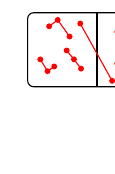
\begin{tikzpicture}[scale=0.25, every node/.style={scale=0.25}, baseline=(current bounding box.center)]
\useasboundingbox (0,-3) rectangle (3,3);
\def\xscale{1} % Horizontal scale factor
\def\yscale{1} % Vertical scale factor
\def\spnt{0.15} % Size of smaller points
\def\lpnt{0.125} % Size of larger points
\draw (3.52*\xscale, 3.76*\yscale) -- (3.52*\xscale, 0);
\draw[rounded corners=2ex*0.25] (0,0) rectangle (7.04*\xscale,3.76*\yscale);
\fill[red] (4.55*\xscale, 1.18*\yscale) circle (\spnt);
\fill[red] (6.05*\xscale, 2.78*\yscale) circle (\spnt);
\draw[red] (4.55*\xscale, 1.18*\yscale) -- (6.05*\xscale,2.78*\yscale);
\fill[red] (4.55*\xscale, 2.79*\yscale) circle (\spnt);
\fill[red] (6.05*\xscale, 1.12*\yscale) circle (\spnt);
\draw[red] (4.55*\xscale, 2.79*\yscale) -- (6.05*\xscale,1.12*\yscale);
\fill[red] (2.67*\xscale, 3.21*\yscale) circle (\spnt);
\fill[red] (4.29*\xscale, 0.3*\yscale) circle (\spnt);
\draw[red] (2.67*\xscale, 3.21*\yscale) -- (4.29*\xscale,0.3*\yscale);
\fill[red] (1.09*\xscale, 3.07*\yscale) circle (\spnt);
\fill[red] (1.526001050877835*\xscale, 3.393088634545991*\yscale) circle (\spnt);
\fill[red] (2.13*\xscale, 2.55*\yscale) circle (\spnt);
\draw[red] (1.09*\xscale, 3.07*\yscale) -- (1.526001050877835*\xscale,3.393088634545991*\yscale) -- (2.13*\xscale,2.55*\yscale);
\fill[red] (0.64*\xscale, 1.39*\yscale) circle (\spnt);
\fill[red] (1.01*\xscale, 0.79*\yscale) circle (\spnt);
\fill[red] (1.35*\xscale, 1.03*\yscale) circle (\spnt);
\draw[red] (0.64*\xscale, 1.39*\yscale) -- (1.01*\xscale,0.79*\yscale) -- (1.35*\xscale,1.03*\yscale);
\fill[red] (1.98*\xscale, 1.84*\yscale) circle (\spnt);
\fill[red] (2.3511520552717013*\xscale, 1.3932029657051672*\yscale) circle (\spnt);
\fill[red] (2.71*\xscale, 0.92*\yscale) circle (\spnt);
\draw[red] (1.98*\xscale, 1.84*\yscale) -- (2.3511520552717013*\xscale,1.3932029657051672*\yscale) -- (2.71*\xscale,0.92*\yscale);
\end{tikzpicture} 
}
\newcommand{\ttwo}{%
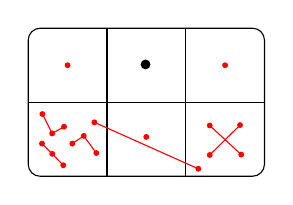
\begin{tikzpicture}[scale=0.5, every node/.style={scale=0.5}]
\def\xscale{1.0} % Horizontal scale factor
\def\yscale{1.0} % Vertical scale factor
\def\spnt{0.075} % Size of smaller points
\def\lpnt{0.125} % Size of larger points
\draw[rounded corners=2ex*0.5] (0,0) rectangle (6*\xscale,3.76*\yscale);
\draw (2.0*\xscale, 3.76*\yscale) -- (2.0*\xscale, 0);
\draw (4.0*\xscale, 3.76*\yscale) -- (4.0*\xscale, 0);
\draw (0, 1.88*\yscale) -- (6.0*\xscale, 1.88*\yscale);
\fill[red] (4.61*\xscale, 0.54*\yscale) circle (\spnt);
\fill[red] (5.38*\xscale, 1.3*\yscale) circle (\spnt);
\draw[red] (4.61*\xscale, 0.54*\yscale) -- (5.38*\xscale,1.3*\yscale);
\fill[red] (1.68*\xscale, 1.37*\yscale) circle (\spnt);
\fill[red] (4.32*\xscale, 0.19*\yscale) circle (\spnt);
\draw[red] (1.68*\xscale, 1.37*\yscale) -- (4.32*\xscale,0.19*\yscale);
\fill[red] (4.61*\xscale, 1.29*\yscale) circle (\spnt);
\fill[red] (5.41*\xscale, 0.55*\yscale) circle (\spnt);
\draw[red] (4.61*\xscale, 1.29*\yscale) -- (5.41*\xscale,0.55*\yscale);
\fill[red] (1.12*\xscale, 0.83*\yscale) circle (\spnt);
\fill[red] (1.4096601986560762*\xscale, 1.0249991174784614*\yscale) circle (\spnt);
\fill[red] (1.73*\xscale, 0.59*\yscale) circle (\spnt);
\draw[red] (1.12*\xscale, 0.83*\yscale) -- (1.4096601986560762*\xscale,1.0249991174784614*\yscale) -- (1.73*\xscale,0.59*\yscale);
\fill[red] (1*\xscale, 2.82*\yscale) circle (\spnt);
\fill[red] (5*\xscale, 2.82*\yscale) circle (\spnt);
\fill[red] (3*\xscale, 1*\yscale) circle (\spnt);
\fill[red] (0.36*\xscale, 1.58*\yscale) circle (\spnt);
\fill[red] (0.6091281492290661*\xscale, 1.0877096738635244*\yscale) circle (\spnt);
\fill[red] (0.91*\xscale, 1.26*\yscale) circle (\spnt);
\draw[red] (0.36*\xscale, 1.58*\yscale) -- (0.6091281492290661*\xscale,1.0877096738635244*\yscale) -- (0.91*\xscale,1.26*\yscale);
\fill[red] (0.35*\xscale, 0.83*\yscale) circle (\spnt);
\fill[red] (0.61*\xscale, 0.57*\yscale) circle (\spnt);
\fill[red] (0.89*\xscale, 0.28*\yscale) circle (\spnt);
\draw[red] (0.35*\xscale, 0.83*\yscale) -- (0.61*\xscale,0.57*\yscale) -- (0.89*\xscale,0.28*\yscale);
\fill (2.98*\xscale,2.84*\yscale) circle (\lpnt);
\end{tikzpicture}
}
\newcommand{\tthree}{%
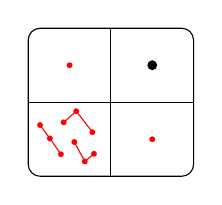
\begin{tikzpicture}[scale=0.5, every node/.style={scale=0.5}]
\def\xscale{1.0} % Horizontal scale factor
\def\yscale{1.0} % Vertical scale factor
\def\spnt{0.075} % Size of smaller points
\def\lpnt{0.125} % Size of larger points
\draw[rounded corners=2ex*0.5] (0,0) rectangle (4.2*\xscale,3.76*\yscale);
\draw (2.1*\xscale, 3.76*\yscale) -- (2.1*\xscale, 0);
\draw (0, 1.88*\yscale) -- (4.2*\xscale, 1.88*\yscale);
\fill[red] (1.05*\xscale, 2.82*\yscale) circle (\spnt);
\fill[red] (3.15*\xscale, 0.94*\yscale) circle (\spnt);
\fill[red] (0.9*\xscale, 1.37*\yscale) circle (\spnt);
\fill[red] (1.2199471753311761*\xscale, 1.6524363073940609*\yscale) circle (\spnt);
\fill[red] (1.63*\xscale, 1.12*\yscale) circle (\spnt);
\draw[red] (0.9*\xscale, 1.37*\yscale) -- (1.2199471753311761*\xscale,1.6524363073940609*\yscale) -- (1.63*\xscale,1.12*\yscale);
\fill[red] (1.17*\xscale, 0.87*\yscale) circle (\spnt);
\fill[red] (1.436829177631258*\xscale, 0.37686266458866924*\yscale) circle (\spnt);
\fill[red] (1.67*\xscale, 0.57*\yscale) circle (\spnt);
\draw[red] (1.17*\xscale, 0.87*\yscale) -- (1.436829177631258*\xscale,0.37686266458866924*\yscale) -- (1.67*\xscale,0.57*\yscale);
\fill[red] (0.3*\xscale, 1.3*\yscale) circle (\spnt);
\fill[red] (0.55*\xscale, 0.96*\yscale) circle (\spnt);
\fill[red] (0.83*\xscale, 0.56*\yscale) circle (\spnt);
\draw[red] (0.3*\xscale, 1.3*\yscale) -- (0.55*\xscale,0.96*\yscale) -- (0.83*\xscale,0.56*\yscale);
\fill (3.150000000000005*\xscale,2.8210223642172525*\yscale) circle (\lpnt);
\end{tikzpicture}
}
\newcommand{\tfour}{%
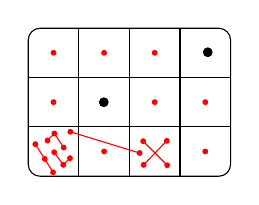
\begin{tikzpicture}[scale=0.5, every node/.style={scale=0.5}]
\def\xscale{1.0} % Horizontal scale factor
\def\yscale{1.0} % Vertical scale factor
\def\spnt{0.075} % Size of smaller points
\def\lpnt{0.125} % Size of larger points
\draw[rounded corners=2ex*0.5] (0,0) rectangle (5.14*\xscale,3.76*\yscale);
\draw (1.285*\xscale, 3.76*\yscale) -- (1.285*\xscale, 0);
\draw (2.57*\xscale, 3.76*\yscale) -- (2.57*\xscale, 0);
\draw (3.855*\xscale, 3.76*\yscale) -- (3.855*\xscale, 0);
\draw (0, 1.2533333333333332*\yscale) -- (5.14*\xscale, 1.2533333333333332*\yscale);
\draw (0, 2.5066666666666664*\yscale) -- (5.14*\xscale, 2.5066666666666664*\yscale);
\fill[red] ({(0*1.285+0.6425)*\xscale}, {(1*1.253+0.63)*\yscale}) circle (\spnt);
\fill[red] ({(0*1.285+0.6425)*\xscale}, {(2*1.253+0.63)*\yscale}) circle (\spnt);
\fill[red] ({(1*1.285+0.6425)*\xscale}, {(0*1.253+0.63)*\yscale}) circle (\spnt);
\fill[red] ({(1*1.285+0.6425)*\xscale}, {(2*1.253+0.63)*\yscale}) circle (\spnt);
\fill[red] ({(2*1.285+0.6425)*\xscale}, {(1*1.253+0.63)*\yscale}) circle (\spnt);
\fill[red] ({(2*1.285+0.6425)*\xscale}, {(2*1.253+0.63)*\yscale}) circle (\spnt);
\fill[red] ({(3*1.285+0.6425)*\xscale}, {(0*1.253+0.63)*\yscale}) circle (\spnt);
\fill[red] ({(3*1.285+0.6425)*\xscale}, {(1*1.253+0.63)*\yscale}) circle (\spnt);
\fill[red] (2.93*\xscale, 0.29*\yscale) circle (\spnt);
\fill[red] (3.52*\xscale, 0.9*\yscale) circle (\spnt);
\draw[red] (2.93*\xscale, 0.29*\yscale) -- (3.52*\xscale,0.9*\yscale);
\fill[red] (1.07*\xscale, 1.13*\yscale) circle (\spnt);
\fill[red] (2.83*\xscale, 0.59*\yscale) circle (\spnt);
\draw[red] (1.07*\xscale, 1.13*\yscale) -- (2.83*\xscale,0.59*\yscale);
\fill[red] (2.92*\xscale, 0.89*\yscale) circle (\spnt);
\fill[red] (3.53*\xscale, 0.28*\yscale) circle (\spnt);
\draw[red] (2.92*\xscale, 0.89*\yscale) -- (3.53*\xscale,0.28*\yscale);
\fill[red] (0.49*\xscale, 0.91*\yscale) circle (\spnt);
\fill[red] (0.6644210751853692*\xscale, 1.086774200246225*\yscale) circle (\spnt);
\fill[red] (0.9*\xscale, 0.73*\yscale) circle (\spnt);
\draw[red] (0.49*\xscale, 0.91*\yscale) -- (0.6644210751853692*\xscale,1.086774200246225*\yscale) -- (0.9*\xscale,0.73*\yscale);
\fill[red] (0.66*\xscale, 0.61*\yscale) circle (\spnt);
\fill[red] (0.89*\xscale, 0.29*\yscale) circle (\spnt);
\fill[red] (1.06*\xscale, 0.46*\yscale) circle (\spnt);
\draw[red] (0.66*\xscale, 0.61*\yscale) -- (0.89*\xscale,0.29*\yscale) -- (1.06*\xscale,0.46*\yscale);
\fill[red] (0.18033887520734232*\xscale, 0.816133743581277*\yscale) circle (\spnt);
\fill[red] (0.42*\xscale, 0.44*\yscale) circle (\spnt);
\fill[red] (0.63*\xscale, 0.1*\yscale) circle (\spnt);
\draw[red] (0.18033887520734232*\xscale, 0.816133743581277*\yscale) -- (0.42*\xscale,0.44*\yscale) -- (0.63*\xscale,0.1*\yscale);
\fill (1.92*\xscale,1.88*\yscale) circle (\lpnt);
\fill (4.56*\xscale,3.15*\yscale) circle (\lpnt);
\end{tikzpicture}
}
\newcommand{\tpair}{%
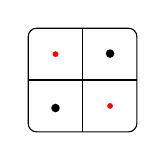
\begin{tikzpicture}[scale=0.35, every node/.style={scale=0.35}, baseline=(current bounding box.center)]
\def\xscale{1.0} % Horizontal scale factor
\def\yscale{1.0} % Vertical scale factor
\def\spnt{0.105} % Size of smaller points
\def\lpnt{0.155} % Size of larger points
\draw[rounded corners=2ex*.35] (0,0) rectangle (3.94*\xscale,3.76*\yscale);
\draw (1.97*\xscale, 3.76*\yscale) -- (1.97*\xscale, 0);
\draw (0, 1.88*\yscale) -- (3.94*\xscale, 1.88*\yscale);
\fill (0.99*\xscale,0.864920127795527*\yscale) circle (\lpnt);
\fill (2.97*\xscale,2.841054313099042*\yscale) circle (\lpnt);
\fill[red] (0.99*\xscale,3.76*0.75*\yscale) circle (\spnt);
\fill[red] (3*0.99*\xscale,3.76*0.25*\yscale) circle (\spnt);
\end{tikzpicture}
}
\begin{center}
\scalebox{1}{\begin{tikzpicture}
    \node (root) at (-0.5, 0) {\tone};
    \node (lvl_1_1) at (-3,-2.25) {\ttwo};
    \node (lvl_1_2) at (0,-2.25) {\tnodeempty};
    \node (lvl_1_3) at (3,-2.25) {\tthree};
    
    \node (lvl_2_1) at (-4.5,-5.5) {\tone};
    \node (lvl_2_2) at (-2, -5.5) {\todesingle{\point{0.08}}};
    
    \node (lvl_2_3) at (1.75,-5.5) {\tfour};
    \node (lvl_2_4) at (4.25,-5.5) {\todesingle{\point{0.08}}};
    
    \node (lvl_3_1) at (0,-9) {\tone};
    \node (lvl_3_2) at (3.25,-8.73) {\tpair};
    
    \node (lvl_4_1) at (2,-11.75) {\todesingle{\point{0.08}}};
    \node (lvl_4_2) at (4.5,-11.75) {\todesingle{\point{0.08}}};
    
    \ptedge{(root)}{(0,1.2)}{(lvl_1_1)}{(-0.5,1.3)}
    \ptedge{(root)}{(0,1.2)}{(lvl_1_2)}{(-0.5,1.3)}
    \ptedge{(root)}{(0,1.2)}{(lvl_1_3)}{(-0.5,1.3)}
    
    \ptedge{(lvl_1_1)}{(-0.5,0.25)}{(lvl_2_1)}{(0,1.3)}
    \ptedge{(lvl_1_1)}{(-0.5,0.25)}{(lvl_2_2)}{(-0.5,1.3)}
    \ptedge{(lvl_1_3)}{(-0.5,0.25)}{(lvl_2_3)}{(-0.5,1.3)}
    \ptedge{(lvl_1_3)}{(-0.5,0.25)}{(lvl_2_4)}{(-0.5,1.3)}
    
    \ptedge{(lvl_2_3)}{(-0.5,0.25)}{(lvl_3_1)}{(0,1.3)}
    \ptedge{(lvl_2_3)}{(-0.5,0.25)}{(lvl_3_2)}{(-0.5,1.02)}
    
    
    \ptedge{(lvl_3_2)}{(-0.5,0.53)}{(lvl_4_1)}{(-0.5,1.3)}
    \ptedge{(lvl_3_2)}{(-0.5,0.53)}{(lvl_4_2)}{(-0.5,1.3)}
\end{tikzpicture}}
\end{center}
}
    \vspace*{-14mm}
    \caption{The tree representation of the formal grammar of the specification found for $\textsf{Av}_{\geq1}(231,312,321)$ after placing and factoring out the top point.}
    \label{fig:fibpermtree}
\end{figure}

\section{Permutation classes}
The experiments we carried out can be separated into known Wilf classes and \emph{experimental classes}.

The experiments for known Wilf classes includes bijections found for all the permutation classes shown to be Wilf classes with bijections in \authcite{simionandschmidt}, excluding symmetries. These classes are split over the next five subsections.

An experimental class is a collection of permutation classes that share the first $12$ terms in their counting sequence. For the experimental classes we focused on classes avoiding patterns of size $4$. We started with those avoiding eleven patterns and worked our way downwards. Symmetries and classes with a \emph{regular insertion encoding}, defined in \authcite{albert2005insertion}, were omitted.


\subsection{Avoiding one pattern of size 3}\label{ss:onexthree}
The parallel specification we found for $\Av{123}$ and $\Av{132}$ have an identical tree structure and even share strategies. They are 
\begin{align*}
    \spec{C} = \left(
        \begin{pmatrix}
            \mathcal{C}^{(1)}\\
            \mathcal{C}^{(2)}\\
            \mathcal{C}^{(3)}\\
            \mathcal{C}^{(4)}\\
            \mathcal{C}^{(5)}\\
            \mathcal{C}^{(6)}\\
            \mathcal{C}^{(7)}
        \end{pmatrix}
        \begin{matrix}\\ \\ \\ \\ \\ \\ ,\end{matrix}
        \begin{pmatrix}
            o_1\\
            o_2\\
            o_3\\
            o_4\\
            o_5\\
            o_6\\
            o_7
        \end{pmatrix}
        \begin{matrix}\\ \\ \\ \\ \\ \\ ,\end{matrix}
        \begin{pmatrix}
            \set{\varepsilon} & \mathcal{C}^{(2)} & \emptyset\\
            \mathcal{C}^{(3)} & \set{1} & \emptyset\\
            \mathcal{C}^{(4)} & \emptyset & \emptyset\\
            \set{\varepsilon} & \mathcal{C}^{(5)} & \mathcal{C}^{(6)}\\
            \mathcal{C}^{(7)} & \set{1} & \emptyset\\
            \mathcal{C}^{(4)} & \mathcal{C}^{(8)} & \emptyset\\
            \mathcal{C}^{(4)} & \emptyset & \emptyset
        \end{pmatrix}
        \begin{matrix}\\ \\ \\ \\ \\ \\ ,\end{matrix}
        \begin{pmatrix}
        2\\
        2\\
        1\\
        3\\
        2\\
        2\\
        1
        \end{pmatrix}
    \right)
\end{align*}
and
\begin{align*}
    \spec{D} = \left(
        \begin{pmatrix}
            \mathcal{D}^{(1)}\\
            \mathcal{D}^{(2)}\\
            \mathcal{D}^{(3)}\\
            \mathcal{D}^{(4)}\\
            \mathcal{D}^{(5)}\\
            \mathcal{D}^{(6)}\\
            \mathcal{D}^{(7)}
        \end{pmatrix}
        \begin{matrix}\\ \\ \\ \\ \\ \\ ,\end{matrix}
        \begin{pmatrix}
            o_1\\
            o_2\\
            o_3\\
            o_4\\
            o_5\\
            o_6\\
            o_7
        \end{pmatrix}
        \begin{matrix}\\ \\ \\ \\ \\ \\ ,\end{matrix}
        \begin{pmatrix}
            \set{\varepsilon} & \mathcal{D}^{(2)} & \emptyset\\
            \mathcal{D}^{(3)} & \set{1} & \emptyset\\
            \mathcal{D}^{(4)} & \emptyset & \emptyset\\
            \set{\varepsilon} & \mathcal{D}^{(5)} & \mathcal{D}^{(6)}\\
            \mathcal{D}^{(7)} & \set{1} & \emptyset\\
            \mathcal{D}^{(4)} & \mathcal{D}^{(8)} & \emptyset\\
            \mathcal{D}^{(4)} & \emptyset & \emptyset
        \end{pmatrix}
        \begin{matrix}\\ \\ \\ \\ \\ \\ ,\end{matrix}
        \begin{pmatrix}
        2\\
        2\\
        1\\
        3\\
        2\\
        2\\
        1
        \end{pmatrix}
    \right)
\end{align*}
where classes are listed in \TableRef{tab:ssclasses} in matched pairs and the constructor's rules can be seen in \TableRef{tab:av123av132constructors}.

\begin{table}[ht!]
    \centering
    {
\newcommand{\tablewrap}[1]{\begin{tabular}{c}#1\end{tabular}}
\newcommand{\tablewraptwo}[2]{\begin{tabular}{c}#2\\#1\end{tabular}}

% ROOT 

\newcommand{\AONE}[2]{\begin{tikzpicture}[scale=#1, every node/.style={scale=#1}]
\def\xscale{1.0} % Horizontal scale factor
\def\yscale{1.0} % Vertical scale factor
\def\spnt{0.075*#2} % Size of smaller points
\def\lpnt{0.125*#2} % Size of larger points
\def\roundscale{0.5} % The rounding factor
\draw[rounded corners=2ex*\roundscale] (0,0) rectangle (4.0*\xscale,4.0*\yscale);
\fill[red] (1.01*\xscale, 1.03*\yscale) circle (\spnt);
\fill[red] (2.05*\xscale, 2.01*\yscale) circle (\spnt);
\fill[red] (3.02*\xscale, 2.93*\yscale) circle (\spnt);
\draw[red] (1.01*\xscale, 1.03*\yscale) -- (2.05*\xscale,2.01*\yscale) -- (3.02*\xscale,2.93*\yscale);
\end{tikzpicture}}

\newcommand{\BONE}[2]{\begin{tikzpicture}[scale=#1, every node/.style={scale=#1}]
\def\xscale{1.0} % Horizontal scale factor
\def\yscale{1.0} % Vertical scale factor
\def\spnt{0.075*#2} % Size of smaller points
\def\lpnt{0.125*#2} % Size of larger points
\def\roundscale{0.5} % The rounding factor
\draw[rounded corners=2ex*\roundscale] (0,0) rectangle (4.0*\xscale,4.0*\yscale);
\fill[red] (0.8716573396242947*\xscale, 1.0019086145039522*\yscale) circle (\spnt);
\fill[red] (2.165701642136188*\xscale, 3.0754616857922144*\yscale) circle (\spnt);
\fill[red] (3.146447488953841*\xscale, 2.172826722776084*\yscale) circle (\spnt);
\draw[red] (0.8716573396242947*\xscale, 1.0019086145039522*\yscale) -- (2.165701642136188*\xscale,3.0754616857922144*\yscale) -- (3.146447488953841*\xscale,2.172826722776084*\yscale);
\end{tikzpicture}}

% LVL 1

\newcommand{\ATWO}[2]{\begin{tikzpicture}[scale=#1, every node/.style={scale=#1}]
\def\xscale{1.0} % Horizontal scale factor
\def\yscale{1.0} % Vertical scale factor
\def\spnt{0.075*#2} % Size of smaller points
\def\lpnt{0.125*#2} % Size of larger points
\def\roundscale{0.5} % The rounding factor
\fill[red] (6.0*\xscale,6.0*\yscale) circle (\spnt);
\fill[red] (10.0*\xscale,2.0*\yscale) circle (\spnt);
\fill[red] (2.0*\xscale,2.0*\yscale) circle (\spnt);
\draw[rounded corners=2ex*\roundscale] (0,0) rectangle (12.0*\xscale,8.0*\yscale);
\draw (4.0*\xscale, 8.0*\yscale) -- (4.0*\xscale, 0);
\draw (8.0*\xscale, 8.0*\yscale) -- (8.0*\xscale, 0);
\draw (0, 4.0*\yscale) -- (12.0*\xscale, 4.0*\yscale);
\fill[red] (9.4*\xscale, 5.02*\yscale) circle (\spnt);
\fill[red] (10.91*\xscale, 6.35*\yscale) circle (\spnt);
\draw[red] (9.4*\xscale, 5.02*\yscale) -- (10.91*\xscale,6.35*\yscale);
\fill[red] (1.05*\xscale, 4.49*\yscale) circle (\spnt);
\fill[red] (2.24*\xscale, 5.14*\yscale) circle (\spnt);
\fill[red] (3.4284957400417544*\xscale, 5.739789457224862*\yscale) circle (\spnt);
\draw[red] (1.05*\xscale, 4.49*\yscale) -- (2.24*\xscale,5.14*\yscale) -- (3.4284957400417544*\xscale,5.739789457224862*\yscale);
\fill[red] (0.81*\xscale, 5.92*\yscale) circle (\spnt);
\fill[red] (3.09*\xscale, 6.32*\yscale) circle (\spnt);
\fill[red] (9.549682814183685*\xscale, 7.419343648657292*\yscale) circle (\spnt);
\draw[red] (0.81*\xscale, 5.92*\yscale) -- (3.09*\xscale,6.32*\yscale) -- (9.549682814183685*\xscale,7.419343648657292*\yscale);
\fill (5.99*\xscale,1.96*\yscale) circle (\lpnt);
\end{tikzpicture}}

\newcommand{\BTWO}[2]{\begin{tikzpicture}[scale=#1, every node/.style={scale=#1}]
\def\xscale{1.0} % Horizontal scale factor
\def\yscale{1.0} % Vertical scale factor
\def\spnt{0.075*#2} % Size of smaller points
\def\lpnt{0.125*#2} % Size of larger points
\def\roundscale{0.5} % The rounding factor
\fill[red] (6.0*\xscale,6.0*\yscale) circle (\spnt);
\fill[red] (10.0*\xscale,2.0*\yscale) circle (\spnt);
\fill[red] (2.0*\xscale,2.0*\yscale) circle (\spnt);
\draw[rounded corners=2ex*\roundscale] (0,0) rectangle (12.0*\xscale,8.0*\yscale);
\draw (4.0*\xscale, 8.0*\yscale) -- (4.0*\xscale, 0);
\draw (8.0*\xscale, 8.0*\yscale) -- (8.0*\xscale, 0);
\draw (0, 4.0*\yscale) -- (12.0*\xscale, 4.0*\yscale);
\fill[red] (8.682948436047251*\xscale, 5.949925271773672*\yscale) circle (\spnt);
\fill[red] (10.428201662843525*\xscale, 4.665194343339079*\yscale) circle (\spnt);
\draw[red] (8.682948436047251*\xscale, 5.949925271773672*\yscale) -- (10.428201662843525*\xscale,4.665194343339079*\yscale);
\fill[red] (0.51*\xscale, 5.31*\yscale) circle (\spnt);
\fill[red] (1.26*\xscale, 6.95*\yscale) circle (\spnt);
\fill[red] (2.21*\xscale, 6.21*\yscale) circle (\spnt);
\draw[red] (0.51*\xscale, 5.31*\yscale) -- (1.26*\xscale,6.95*\yscale) -- (2.21*\xscale,6.21*\yscale);
\fill[red] (2.2*\xscale, 4.62*\yscale) circle (\spnt);
\fill[red] (3.39*\xscale, 7.41*\yscale) circle (\spnt);
\fill[red] (10.68*\xscale, 6.19*\yscale) circle (\spnt);
\draw[red] (2.2*\xscale, 4.62*\yscale) -- (3.39*\xscale,7.41*\yscale) -- (10.68*\xscale,6.19*\yscale);
\fill (6.04*\xscale,1.97*\yscale) circle (\lpnt);
\end{tikzpicture}}

% LVL 2

\newcommand{\ATHREE}[2]{\begin{tikzpicture}[scale=#1, every node/.style={scale=#1}]
\def\xscale{1.0} % Horizontal scale factor
\def\yscale{1.0} % Vertical scale factor
\def\spnt{0.075*#2} % Size of smaller points
\def\lpnt{0.125*#2} % Size of larger points
\def\roundscale{0.5} % The rounding factor
\draw[rounded corners=2ex*\roundscale] (0,0) rectangle (8.0*\xscale,4.0*\yscale);
\draw (4.0*\xscale, 4.0*\yscale) -- (4.0*\xscale, 0);
\fill[red] (5.598960089839087*\xscale, 0.9002276274053245*\yscale) circle (\spnt);
\fill[red] (7.04*\xscale, 1.67*\yscale) circle (\spnt);
\draw[red] (5.598960089839087*\xscale, 0.9002276274053245*\yscale) -- (7.04*\xscale,1.67*\yscale);
\fill[red] (0.76*\xscale, 1.88*\yscale) circle (\spnt);
\fill[red] (1.88*\xscale, 2.44*\yscale) circle (\spnt);
\fill[red] (2.97*\xscale, 2.97*\yscale) circle (\spnt);
\draw[red] (0.76*\xscale, 1.88*\yscale) -- (1.88*\xscale,2.44*\yscale) -- (2.97*\xscale,2.97*\yscale);
\fill[red] (1.44*\xscale, 0.87*\yscale) circle (\spnt);
\fill[red] (2.97*\xscale, 1.59*\yscale) circle (\spnt);
\fill[red] (6.029333567440057*\xscale, 2.98047911380251*\yscale) circle (\spnt);
\draw[red] (1.44*\xscale, 0.87*\yscale) -- (2.97*\xscale,1.59*\yscale) -- (6.029333567440057*\xscale,2.98047911380251*\yscale);
\end{tikzpicture}}

\newcommand{\BTHREE}[2]{\begin{tikzpicture}[scale=#1, every node/.style={scale=#1}]
\def\xscale{1.0} % Horizontal scale factor
\def\yscale{1.0} % Vertical scale factor
\def\spnt{0.075*#2} % Size of smaller points
\def\lpnt{0.125*#2} % Size of larger points
\def\roundscale{0.5} % The rounding factor
\draw[rounded corners=2ex*\roundscale] (0,0) rectangle (8.0*\xscale,4.0*\yscale);
\draw (4.0*\xscale, 4.0*\yscale) -- (4.0*\xscale, 0);
\fill[red] (5.854277604508614*\xscale, 3.237297302338969*\yscale) circle (\spnt);
\fill[red] (7.218773962502269*\xscale, 1.979962497743513*\yscale) circle (\spnt);
\draw[red] (5.854277604508614*\xscale, 3.237297302338969*\yscale) -- (7.218773962502269*\xscale,1.979962497743513*\yscale);
\fill[red] (0.7800987765155368*\xscale, 1.4844050917510438*\yscale) circle (\spnt);
\fill[red] (1.514406103733271*\xscale, 3.2931924028795447*\yscale) circle (\spnt);
\fill[red] (2.66*\xscale, 2.5*\yscale) circle (\spnt);
\draw[red] (0.7800987765155368*\xscale, 1.4844050917510438*\yscale) -- (1.514406103733271*\xscale,3.2931924028795447*\yscale) -- (2.66*\xscale,2.5*\yscale);
\fill[red] (2.56*\xscale, 0.99*\yscale) circle (\spnt);
\fill[red] (3.58*\xscale, 3.04*\yscale) circle (\spnt);
\fill[red] (5.77*\xscale, 1.6370373134954155*\yscale) circle (\spnt);
\draw[red] (2.56*\xscale, 0.99*\yscale) -- (3.58*\xscale,3.04*\yscale) -- (5.77*\xscale,1.6370373134954155*\yscale);
\end{tikzpicture}}

% LVL 3

\newcommand{\AFOUR}[2]{\begin{tikzpicture}[scale=#1, every node/.style={scale=#1}]
\def\xscale{1.0} % Horizontal scale factor
\def\yscale{1.0} % Vertical scale factor
\def\spnt{0.075*#2} % Size of smaller points
\def\lpnt{0.125*#2} % Size of larger points
\def\roundscale{0.5} % The rounding factor
\fill[green!20,rounded corners=2ex*\roundscale] (4*\xscale,0) rectangle (8.0*\xscale,4.0*\yscale);
\fill[green!20] (4*\xscale,0) rectangle (6*\xscale,4*\yscale);
\draw[rounded corners=2ex*\roundscale] (0,0) rectangle (8.0*\xscale,4.0*\yscale);
\draw (4.0*\xscale, 4.0*\yscale) -- (4.0*\xscale, 0);
\fill[red] (5.598960089839087*\xscale, 0.9002276274053245*\yscale) circle (\spnt);
\fill[red] (7.04*\xscale, 1.67*\yscale) circle (\spnt);
\draw[red] (5.598960089839087*\xscale, 0.9002276274053245*\yscale) -- (7.04*\xscale,1.67*\yscale);
\fill[red] (0.76*\xscale, 1.88*\yscale) circle (\spnt);
\fill[red] (1.88*\xscale, 2.44*\yscale) circle (\spnt);
\fill[red] (2.97*\xscale, 2.97*\yscale) circle (\spnt);
\draw[red] (0.76*\xscale, 1.88*\yscale) -- (1.88*\xscale,2.44*\yscale) -- (2.97*\xscale,2.97*\yscale);
\fill[red] (1.44*\xscale, 0.87*\yscale) circle (\spnt);
\fill[red] (2.97*\xscale, 1.59*\yscale) circle (\spnt);
\fill[red] (6.029333567440057*\xscale, 2.98047911380251*\yscale) circle (\spnt);
\draw[red] (1.44*\xscale, 0.87*\yscale) -- (2.97*\xscale,1.59*\yscale) -- (6.029333567440057*\xscale,2.98047911380251*\yscale);
\end{tikzpicture}}

\newcommand{\BFOUR}[2]{\begin{tikzpicture}[scale=#1, every node/.style={scale=#1}]
\def\xscale{1.0} % Horizontal scale factor
\def\yscale{1.0} % Vertical scale factor
\def\spnt{0.075*#2} % Size of smaller points
\def\lpnt{0.125*#2} % Size of larger points
\def\roundscale{0.5} % The rounding factor
\fill[green!20,rounded corners=2ex*\roundscale] (4*\xscale,0) rectangle (8.0*\xscale,4.0*\yscale);
\fill[green!20] (4*\xscale,0) rectangle (6*\xscale,4*\yscale);
\draw[rounded corners=2ex*\roundscale] (0,0) rectangle (8.0*\xscale,4.0*\yscale);
\draw (4.0*\xscale, 4.0*\yscale) -- (4.0*\xscale, 0);
\fill[red] (5.854277604508614*\xscale, 3.237297302338969*\yscale) circle (\spnt);
\fill[red] (7.218773962502269*\xscale, 1.979962497743513*\yscale) circle (\spnt);
\draw[red] (5.854277604508614*\xscale, 3.237297302338969*\yscale) -- (7.218773962502269*\xscale,1.979962497743513*\yscale);
\fill[red] (0.7800987765155368*\xscale, 1.4844050917510438*\yscale) circle (\spnt);
\fill[red] (1.514406103733271*\xscale, 3.2931924028795447*\yscale) circle (\spnt);
\fill[red] (2.66*\xscale, 2.5*\yscale) circle (\spnt);
\draw[red] (0.7800987765155368*\xscale, 1.4844050917510438*\yscale) -- (1.514406103733271*\xscale,3.2931924028795447*\yscale) -- (2.66*\xscale,2.5*\yscale);
\fill[red] (2.56*\xscale, 0.99*\yscale) circle (\spnt);
\fill[red] (3.58*\xscale, 3.04*\yscale) circle (\spnt);
\fill[red] (5.77*\xscale, 1.6370373134954155*\yscale) circle (\spnt);
\draw[red] (2.56*\xscale, 0.99*\yscale) -- (3.58*\xscale,3.04*\yscale) -- (5.77*\xscale,1.6370373134954155*\yscale);
\end{tikzpicture}}

% LVL 4 - 1

\newcommand{\AFIVE}[2]{\begin{tikzpicture}[scale=#1, every node/.style={scale=#1}]
\def\xscale{1.0} % Horizontal scale factor
\def\yscale{1.0} % Vertical scale factor
\def\spnt{0.075*#2} % Size of smaller points
\def\lpnt{0.125*#2} % Size of larger points
\def\roundscale{0.5} % The rounding factor
\fill[red] (6.0*\xscale,6.0*\yscale) circle (\spnt);
\fill[red] (10.0*\xscale,2.0*\yscale) circle (\spnt);
\fill[red] (14.0*\xscale,2.0*\yscale) circle (\spnt);
\fill[red] (2.0*\xscale,2.0*\yscale) circle (\spnt);
\fill[green!20, rounded corners=2ex*\roundscale] (12*\xscale,4*\yscale) rectangle (16.0*\xscale,8.0*\yscale);
\fill[green!20] (12*\xscale,4*\yscale) rectangle (14.0*\xscale,8.0*\yscale);
\draw[rounded corners=2ex*\roundscale] (0,0) rectangle (16.0*\xscale,8.0*\yscale);
\draw (4.0*\xscale, 8.0*\yscale) -- (4.0*\xscale, 0);
\draw (8.0*\xscale, 8.0*\yscale) -- (8.0*\xscale, 0);
\draw (12.0*\xscale, 8.0*\yscale) -- (12.0*\xscale, 0);
\draw (0, 4.0*\yscale) -- (16.0*\xscale, 4.0*\yscale);
\fill[red] (9.801112294950762*\xscale, 4.87433400586728*\yscale) circle (\spnt);
\fill[red] (11.435748036487725*\xscale, 6.031005179302951*\yscale) circle (\spnt);
\draw[red] (9.801112294950762*\xscale, 4.87433400586728*\yscale) -- (11.435748036487725*\xscale,6.031005179302951*\yscale);
\fill[red] (10.625978487198118*\xscale, 4.71691728339242*\yscale) circle (\spnt);
\fill[red] (14.204868883096946*\xscale, 6.149917253543268*\yscale) circle (\spnt);
\draw[red] (10.625978487198118*\xscale, 4.71691728339242*\yscale) -- (14.204868883096946*\xscale,6.149917253543268*\yscale);
\fill[red] (13.595631280437269*\xscale, 4.61944982640392*\yscale) circle (\spnt);
\fill[red] (15.042199599259325*\xscale, 5.8848845525829105*\yscale) circle (\spnt);
\draw[red] (13.595631280437269*\xscale, 4.61944982640392*\yscale) -- (15.042199599259325*\xscale,5.8848845525829105*\yscale);
\fill[red] (0.82*\xscale, 5.85*\yscale) circle (\spnt);
\fill[red] (1.87*\xscale, 6.66*\yscale) circle (\spnt);
\fill[red] (3.038470356788786*\xscale, 7.538371658226805*\yscale) circle (\spnt);
\draw[red] (0.82*\xscale, 5.85*\yscale) -- (1.87*\xscale,6.66*\yscale) -- (3.038470356788786*\xscale,7.538371658226805*\yscale);
\fill[red] (2.18*\xscale, 4.69*\yscale) circle (\spnt);
\fill[red] (3.47*\xscale, 4.93*\yscale) circle (\spnt);
\fill[red] (9.53*\xscale, 6.06*\yscale) circle (\spnt);
\draw[red] (2.18*\xscale, 4.69*\yscale) -- (3.47*\xscale,4.93*\yscale) -- (9.53*\xscale,6.06*\yscale);
\fill[red] (2.2*\xscale, 6.06*\yscale) circle (\spnt);
\fill[red] (3.39*\xscale, 6.2*\yscale) circle (\spnt);
\fill[red] (13.98024739273349*\xscale, 7.380027548539661*\yscale) circle (\spnt);
\draw[red] (2.2*\xscale, 6.06*\yscale) -- (3.39*\xscale,6.2*\yscale) -- (13.98024739273349*\xscale,7.380027548539661*\yscale);
\fill (6.1*\xscale,1.94*\yscale) circle (\lpnt);
\end{tikzpicture}}

\newcommand{\BFIVE}[2]{
\begin{tikzpicture}[scale=#1, every node/.style={scale=#1}]
\def\xscale{1.0} % Horizontal scale factor
\def\yscale{1.0} % Vertical scale factor
\def\spnt{0.075*#2} % Size of smaller points
\def\lpnt{0.125*#2} % Size of larger points
\def\roundscale{0.5} % The rounding factor
\fill[red] (6.0*\xscale,6.0*\yscale) circle (\spnt);
\fill[red] (10.0*\xscale,2.0*\yscale) circle (\spnt);
\fill[red] (14.0*\xscale,2.0*\yscale) circle (\spnt);
\fill[red] (2.0*\xscale,2.0*\yscale) circle (\spnt);
\fill[green!20, rounded corners=2ex*\roundscale] (12*\xscale,4*\yscale) rectangle (16.0*\xscale,8.0*\yscale);
\fill[green!20] (12*\xscale,4*\yscale) rectangle (14.0*\xscale,8.0*\yscale);
\draw[rounded corners=2ex*\roundscale] (0,0) rectangle (16.0*\xscale,8.0*\yscale);
\draw (4.0*\xscale, 8.0*\yscale) -- (4.0*\xscale, 0);
\draw (8.0*\xscale, 8.0*\yscale) -- (8.0*\xscale, 0);
\draw (12.0*\xscale, 8.0*\yscale) -- (12.0*\xscale, 0);
\draw (0, 4.0*\yscale) -- (16.0*\xscale, 4.0*\yscale);
\fill[red] (10.12*\xscale, 7.4*\yscale) circle (\spnt);
\fill[red] (10.96*\xscale, 6.23*\yscale) circle (\spnt);
\draw[red] (10.12*\xscale, 7.4*\yscale) -- (10.96*\xscale,6.23*\yscale);
\fill[red] (11.45*\xscale, 7.5*\yscale) circle (\spnt);
\fill[red] (13.83*\xscale, 6.01*\yscale) circle (\spnt);
\draw[red] (11.45*\xscale, 7.5*\yscale) -- (13.83*\xscale,6.01*\yscale);
\fill[red] (14.49*\xscale, 7.45*\yscale) circle (\spnt);
\fill[red] (15.341775454722875*\xscale, 6.279291533596879*\yscale) circle (\spnt);
\draw[red] (14.49*\xscale, 7.45*\yscale) -- (15.341775454722875*\xscale,6.279291533596879*\yscale);
\fill[red] (0.7*\xscale, 5.86*\yscale) circle (\spnt);
\fill[red] (1.34*\xscale, 7.27*\yscale) circle (\spnt);
\fill[red] (2.1*\xscale, 6.64*\yscale) circle (\spnt);
\draw[red] (0.7*\xscale, 5.86*\yscale) -- (1.34*\xscale,7.27*\yscale) -- (2.1*\xscale,6.64*\yscale);
\fill[red] (2.72*\xscale, 4.52*\yscale) circle (\spnt);
\fill[red] (3.45*\xscale, 5.79*\yscale) circle (\spnt);
\fill[red] (8.52*\xscale, 4.91*\yscale) circle (\spnt);
\draw[red] (2.72*\xscale, 4.52*\yscale) -- (3.45*\xscale,5.79*\yscale) -- (8.52*\xscale,4.91*\yscale);
\fill[red] (1.8062192976217373*\xscale, 4.668919054695671*\yscale) circle (\spnt);
\fill[red] (3.199753219993414*\xscale, 6.868448702576094*\yscale) circle (\spnt);
\fill[red] (12.53*\xscale, 5.3*\yscale) circle (\spnt);
\draw[red] (1.8062192976217373*\xscale, 4.668919054695671*\yscale) -- (3.199753219993414*\xscale,6.868448702576094*\yscale) -- (12.53*\xscale,5.3*\yscale);
\fill (5.97*\xscale,2.04*\yscale) circle (\lpnt);
\end{tikzpicture}}

% LVL 4 - 2

\newcommand{\ASIX}[2]{\begin{tikzpicture}[scale=#1, every node/.style={scale=#1}]
\def\xscale{1.0} % Horizontal scale factor
\def\yscale{1.0} % Vertical scale factor
\def\spnt{0.075*#2} % Size of smaller points
\def\lpnt{0.125*#2} % Size of larger points
\def\roundscale{0.5} % The rounding factor
\fill[red] (6.0*\xscale,2.0*\yscale) circle (\spnt);
\fill[red] (10.0*\xscale,6.0*\yscale) circle (\spnt);
\fill[red] (2.0*\xscale,2.0*\yscale) circle (\spnt);
\fill[green!20,rounded corners=2ex*\roundscale] (8*\xscale,0) rectangle (12.0*\xscale,4.0*\yscale);
\fill[green!20] (8*\xscale,0) rectangle (10.0*\xscale,4.0*\yscale);
\fill[green!20] (4*\xscale,4*\yscale) rectangle (8.0*\xscale,8.0*\yscale);
\draw[rounded corners=2ex*\roundscale] (0,0) rectangle (12.0*\xscale,8.0*\yscale);
\draw (4.0*\xscale, 8.0*\yscale) -- (4.0*\xscale, 0);
\draw (8.0*\xscale, 8.0*\yscale) -- (8.0*\xscale, 0);
\draw (0, 4.0*\yscale) -- (12.0*\xscale, 4.0*\yscale);
\fill[red] (5.34854305480012*\xscale, 5.141934256406755*\yscale) circle (\spnt);
\fill[red] (7.27*\xscale, 6.31*\yscale) circle (\spnt);
\draw[red] (5.34854305480012*\xscale, 5.141934256406755*\yscale) -- (7.27*\xscale,6.31*\yscale);
\fill[red] (1.0*\xscale, 5.95602761572349*\yscale) circle (\spnt);
\fill[red] (2.07*\xscale, 6.49*\yscale) circle (\spnt);
\fill[red] (3.236674307340645*\xscale, 7.080100135433983*\yscale) circle (\spnt);
\draw[red] (1.0*\xscale, 5.95602761572349*\yscale) -- (2.07*\xscale,6.49*\yscale) -- (3.236674307340645*\xscale,7.080100135433983*\yscale);
\fill[red] (1.87*\xscale, 5.12*\yscale) circle (\spnt);
\fill[red] (3.21*\xscale, 5.8*\yscale) circle (\spnt);
\fill[red] (5.08*\xscale, 6.74*\yscale) circle (\spnt);
\draw[red] (1.87*\xscale, 5.12*\yscale) -- (3.21*\xscale,5.8*\yscale) -- (5.08*\xscale,6.74*\yscale);
\fill (10.1*\xscale,2.12*\yscale) circle (\lpnt);
\end{tikzpicture}}

\newcommand{\BSIX}[2]{\begin{tikzpicture}[scale=#1, every node/.style={scale=#1}]
\def\xscale{1.0} % Horizontal scale factor
\def\yscale{1.0} % Vertical scale factor
\def\spnt{0.075*#2} % Size of smaller points
\def\lpnt{0.125*#2} % Size of larger points
\def\roundscale{0.5} % The rounding factor
\fill[red] (6.0*\xscale,6.0*\yscale) circle (\spnt);
\fill[red] (10.0*\xscale,2.0*\yscale) circle (\spnt);
\fill[red] (2.0*\xscale,2.0*\yscale) circle (\spnt);
\fill[green!20,rounded corners=2ex*\roundscale] (8*\xscale,4*\yscale) rectangle (12.0*\xscale,8.0*\yscale);
\fill[green!20] (8*\xscale,4*\yscale) rectangle (10.0*\xscale,8.0*\yscale);
\fill[green!20] (4*\xscale,0) rectangle (8.0*\xscale,4.0*\yscale);
\draw[rounded corners=2ex*\roundscale] (0,0) rectangle (12.0*\xscale,8.0*\yscale);
\draw (4.0*\xscale, 8.0*\yscale) -- (4.0*\xscale, 0);
\draw (8.0*\xscale, 8.0*\yscale) -- (8.0*\xscale, 0);
\draw (0, 4.0*\yscale) -- (12.0*\xscale, 4.0*\yscale);
\fill[red] (8.682948436047251*\xscale, 5.949925271773672*\yscale) circle (\spnt);
\fill[red] (10.428201662843525*\xscale, 4.665194343339079*\yscale) circle (\spnt);
\draw[red] (8.682948436047251*\xscale, 5.949925271773672*\yscale) -- (10.428201662843525*\xscale,4.665194343339079*\yscale);
\fill[red] (0.51*\xscale, 5.31*\yscale) circle (\spnt);
\fill[red] (1.26*\xscale, 6.95*\yscale) circle (\spnt);
\fill[red] (2.21*\xscale, 6.21*\yscale) circle (\spnt);
\draw[red] (0.51*\xscale, 5.31*\yscale) -- (1.26*\xscale,6.95*\yscale) -- (2.21*\xscale,6.21*\yscale);
\fill[red] (2.2*\xscale, 4.62*\yscale) circle (\spnt);
\fill[red] (3.39*\xscale, 7.41*\yscale) circle (\spnt);
\fill[red] (10.68*\xscale, 6.19*\yscale) circle (\spnt);
\draw[red] (2.2*\xscale, 4.62*\yscale) -- (3.39*\xscale,7.41*\yscale) -- (10.68*\xscale,6.19*\yscale);
\fill (6.04*\xscale,1.97*\yscale) circle (\lpnt);
\end{tikzpicture}}

% LVL 5
\newcommand{\ASEVEN}[2]{\begin{tikzpicture}[scale=#1, every node/.style={scale=#1}]
\def\xscale{1.0} % Horizontal scale factor
\def\yscale{1.0} % Vertical scale factor
\def\spnt{0.075*#2} % Size of smaller points
\def\lpnt{0.125*#2} % Size of larger points
\def\roundscale{0.5} % The rounding factor
\fill[green!20, rounded corners=2ex*\roundscale] (8*\xscale,0) rectangle (12.0*\xscale,4.0*\yscale);
\fill[green!20] (10*\xscale,0) rectangle (12.0*\xscale,4.0*\yscale);
\draw[rounded corners=2ex*\roundscale] (0,0) rectangle (12.0*\xscale,4.0*\yscale);
\draw (4.0*\xscale, 4.0*\yscale) -- (4.0*\xscale, 0);
\draw (8.0*\xscale, 4.0*\yscale) -- (8.0*\xscale, 0);
\fill[red] (5.91*\xscale, 0.54*\yscale) circle (\spnt);
\fill[red] (7.33*\xscale, 0.97*\yscale) circle (\spnt);
\draw[red] (5.91*\xscale, 0.54*\yscale) -- (7.33*\xscale,0.97*\yscale);
\fill[red] (6.89*\xscale, 1.31*\yscale) circle (\spnt);
\fill[red] (8.89*\xscale, 1.93*\yscale) circle (\spnt);
\draw[red] (6.89*\xscale, 1.31*\yscale) -- (8.89*\xscale,1.93*\yscale);
\fill[red] (9.5*\xscale, 0.79*\yscale) circle (\spnt);
\fill[red] (11.05*\xscale, 1.36*\yscale) circle (\spnt);
\draw[red] (9.5*\xscale, 0.79*\yscale) -- (11.05*\xscale,1.36*\yscale);
\fill[red] (0.67*\xscale, 2.33*\yscale) circle (\spnt);
\fill[red] (1.91*\xscale, 2.72*\yscale) circle (\spnt);
\fill[red] (3.15*\xscale, 3.09*\yscale) circle (\spnt);
\draw[red] (0.67*\xscale, 2.33*\yscale) -- (1.91*\xscale,2.72*\yscale) -- (3.15*\xscale,3.09*\yscale);
\fill[red] (1.31*\xscale, 1.63*\yscale) circle (\spnt);
\fill[red] (3.29*\xscale, 2.1*\yscale) circle (\spnt);
\fill[red] (6.46*\xscale, 2.85*\yscale) circle (\spnt);
\draw[red] (1.31*\xscale, 1.63*\yscale) -- (3.29*\xscale,2.1*\yscale) -- (6.46*\xscale,2.85*\yscale);
\fill[red] (2.02*\xscale, 1.1*\yscale) circle (\spnt);
\fill[red] (3.33*\xscale, 1.4*\yscale) circle (\spnt);
\fill[red] (10.33*\xscale, 2.97*\yscale) circle (\spnt);
\draw[red] (2.02*\xscale, 1.1*\yscale) -- (3.33*\xscale,1.4*\yscale) -- (10.33*\xscale,2.97*\yscale);
\end{tikzpicture}}

\newcommand{\BSEVEN}[2]{\begin{tikzpicture}[scale=#1, every node/.style={scale=#1}]
\def\xscale{1.0} % Horizontal scale factor
\def\yscale{1.0} % Vertical scale factor
\def\spnt{0.075*#2} % Size of smaller points
\def\lpnt{0.125*#2} % Size of larger points
\def\roundscale{0.5} % The rounding factor
\fill[green!20, rounded corners=2ex*\roundscale] (8*\xscale,0) rectangle (12.0*\xscale,4.0*\yscale);
\fill[green!20] (10*\xscale,0) rectangle (12.0*\xscale,4.0*\yscale);
\draw[rounded corners=2ex*\roundscale] (0,0) rectangle (12.0*\xscale,4.0*\yscale);
\draw (4.0*\xscale, 4.0*\yscale) -- (4.0*\xscale, 0);
\draw (8.0*\xscale, 4.0*\yscale) -- (8.0*\xscale, 0);
\fill[red] (5.75*\xscale, 1.24*\yscale) circle (\spnt);
\fill[red] (7.01*\xscale, 0.84*\yscale) circle (\spnt);
\draw[red] (5.75*\xscale, 1.24*\yscale) -- (7.01*\xscale,0.84*\yscale);
\fill[red] (7.56*\xscale, 2.08*\yscale) circle (\spnt);
\fill[red] (8.71*\xscale, 1.64*\yscale) circle (\spnt);
\draw[red] (7.56*\xscale, 2.08*\yscale) -- (8.71*\xscale,1.64*\yscale);
\fill[red] (9.79*\xscale, 2.04*\yscale) circle (\spnt);
\fill[red] (11.19*\xscale, 1.52*\yscale) circle (\spnt);
\draw[red] (9.79*\xscale, 2.04*\yscale) -- (11.19*\xscale,1.52*\yscale);
\fill[red] (0.58*\xscale, 1.37*\yscale) circle (\spnt);
\fill[red] (1.08*\xscale, 2.86*\yscale) circle (\spnt);
\fill[red] (1.69*\xscale, 2.33*\yscale) circle (\spnt);
\draw[red] (0.58*\xscale, 1.37*\yscale) -- (1.08*\xscale,2.86*\yscale) -- (1.69*\xscale,2.33*\yscale);
\fill[red] (2.54*\xscale, 1.36*\yscale) circle (\spnt);
\fill[red] (3.48*\xscale, 2.36*\yscale) circle (\spnt);
\fill[red] (6.52*\xscale, 1.92*\yscale) circle (\spnt);
\draw[red] (2.54*\xscale, 1.36*\yscale) -- (3.48*\xscale,2.36*\yscale) -- (6.52*\xscale,1.92*\yscale);
\fill[red] (2.46*\xscale, 2.52*\yscale) circle (\spnt);
\fill[red] (3.42*\xscale, 3.46*\yscale) circle (\spnt);
\fill[red] (8.62*\xscale, 2.83*\yscale) circle (\spnt);
\draw[red] (2.46*\xscale, 2.52*\yscale) -- (3.42*\xscale,3.46*\yscale) -- (8.62*\xscale,2.83*\yscale);
\end{tikzpicture}}

% Catalytic atom

\newcommand{\AEIGHT}[2]{\begin{tikzpicture}[scale=#1, every node/.style={scale=#1}]
\def\xscale{1.0} % Horizontal scale factor
\def\yscale{1.0} % Vertical scale factor
\def\spnt{0.075*#2} % Size of smaller points
\def\lpnt{0.125*#2} % Size of larger points
\def\roundscale{0.5} % The rounding factor
\fill[green!20,rounded corners=2ex*\roundscale] (0,0) rectangle (4.0*\xscale,4.0*\yscale);
\draw[rounded corners=2ex*\roundscale] (0,0) rectangle (4.0*\xscale,4.0*\yscale);
\fill (2*\xscale,2*\yscale) circle (\lpnt);
\end{tikzpicture}}

\newcommand{\BEIGHT}[2]{\begin{tikzpicture}[scale=#1, every node/.style={scale=#1}]
\def\xscale{1.0} % Horizontal scale factor
\def\yscale{1.0} % Vertical scale factor
\def\spnt{0.075*#2} % Size of smaller points
\def\lpnt{0.125*#2} % Size of larger points
\def\roundscale{0.5} % The rounding factor
\fill[green!20,rounded corners=2ex*\roundscale] (0,0) rectangle (4.0*\xscale,4.0*\yscale);
\draw[rounded corners=2ex*\roundscale] (0,0) rectangle (4.0*\xscale,4.0*\yscale);
\fill (2*\xscale,2*\yscale) circle (\lpnt);
\end{tikzpicture}}

\begin{tabular}{c|c}
    \tablewrap{Tilings in the specification for $\Av{123}$} & \tablewrap{Tilings in the specification for $\Av{132}$}\\
    \hline & \\[-1ex]
    \tablewraptwo{\AONE{0.4}{1.5}}{$\mathcal{C}^{(1)}$} & \tablewraptwo{\BONE{0.4}{1.5}}{$\mathcal{D}^{(1)}$} \\
    \tablewraptwo{\ATWO{0.3}{2}}{$\mathcal{C}^{(2)}$} & \tablewraptwo{\BTWO{0.3}{2}}{$\mathcal{D}^{(2)}$} \\
    \tablewraptwo{\ATHREE{0.4}{1.7}}{$\mathcal{C}^{(3)}$} & \tablewraptwo{\BTHREE{0.4}{1.7}}{$\mathcal{D}^{(3)}$} \\
    \tablewraptwo{\AFOUR{0.4}{1.7}}{$\mathcal{C}^{(4)}$} & \tablewraptwo{\BFOUR{0.4}{1.7}}{$\mathcal{D}^{(4)}$} \\
    \tablewraptwo{\AFIVE{0.3}{2}}{$\mathcal{C}^{(5)}$} & \tablewraptwo{\BFIVE{0.3}{2}}{$\mathcal{D}^{(5)}$} \\
    \tablewraptwo{\ASIX{0.3}{2}}{$\mathcal{C}^{(6)}$} & \tablewraptwo{\BSIX{0.3}{2}}{$\mathcal{D}^{(6)}$} \\
    \tablewraptwo{\ASEVEN{0.4}{1.7}}{$\mathcal{C}^{(7)}$} & \tablewraptwo{\BSEVEN{0.4}{1.7}}{$\mathcal{D}^{(7)}$} \\
    \tablewraptwo{\AEIGHT{0.4}{1.5}}{$\mathcal{C}^{(8)}$} & \tablewraptwo{\BEIGHT{0.4}{1.5}}{$\mathcal{D}^{(8)}$}
\end{tabular}
}
    \caption{The classes and their matching for the parallel specifications of $\Av{123}$ and $\Av{132}$.}
    \label{tab:ssclasses}
\end{table}

\begin{table}[ht!]
    \centering
    \begin{tabular}{c|l}
    Constructor & Rule\\
    \hline
    $o_1$ & Place bottommost point ($+$) \\
    $o_2$ & Factor ($\times$) \\
    $o_3$ & Add assumption in cell $(1,0)$ \\
    $o_4$ & Place bottommost in row ($+$) \\
    $o_5$ & Factor ($\times$) \\
    $o_6$ & Factor ($\times$) \\
    $o_7$ & Fuse columns $1$ and $2$ \\
\end{tabular}
    \caption{Rules for the parallel specifications of $\Av{123}$ and $\Av{132}$.}
    \label{tab:av123av132constructors}
\end{table}

The inputs and outputs of size $4$ for the bijection are shown in \TableRef{tab:ssexamp} and it seems to agree with the \citeauthor{simionandschmidt} bijection in \cite{simionandschmidt} which we leave as an open problem in Conjecture~\ref{con:ss}.

\begin{table}[ht!]
    \centering
    
    \begin{tabular}{c|c}
        $\textsf{Av}_4(123)$ & $\textsf{Av}_4(132)$\\
        \hline
        $4321$ & $4321$\\
        $3421$ & $3421$\\
        $3241$ & $3241$\\
        $4231$ & $4231$\\
        $2431$ & $2341$\\
        $3214$ & $3214$\\
        $4213$ & $4213$\\
        $2413$ & $2314$\\
        $4312$ & $4312$\\
        $3412$ & $3412$\\
        $2143$ & $2134$\\
        $3142$ & $3124$\\
        $4132$ & $4123$\\
        $1432$ & $1234$\\
    \end{tabular}
    \caption{The inputs and outputs of size $4$ for the bijection between $123$ and $132$ avoiding permutations.}
    \label{tab:ssexamp}
\end{table}

\subsection{Avoiding two patterns of size 3}
The only Wilf class with more than one permutation class is the class consisting of $\Av{123,132}$, $\Av{132,213}$ and $\Av{132,231}$. The connections created by bijections found can be seen in \FigureRef{fig:2x3bi}.

\begin{figure}[ht!]
    \centering
    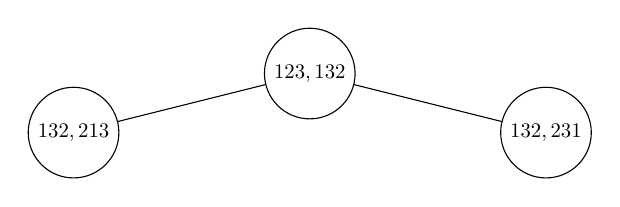
\begin{tikzpicture}[vertex/.style = {shape=circle,draw,minimum size=1.5em},scale=0.75, every node/.style={scale=0.75}]
    \node[vertex] (a) at (0,1) {$\Av{123,132}$};
    \node[vertex] (b) at (-4,0) {$\Av{132,213}$};
    \node[vertex] (c) at (4,0) {$\Av{132,231}$};
    \draw (a) to (b);
    \draw (a) to (c);
\end{tikzpicture}
    \caption{The connections created by bijections found for classes avoiding two patterns of size $3$.}
    \label{fig:2x3bi}
\end{figure}

\subsection{Avoiding three patterns of size 3}
The connections created by bijections found for the only Wilf class (containing more than one permutation class) can be seen in \FigureRef{fig:3x3bi}. 
\begin{figure}[ht!]
    \centering
    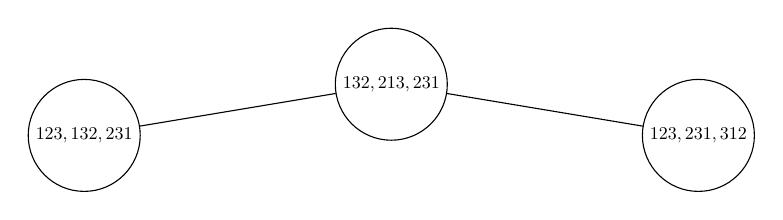
\begin{tikzpicture}[vertex/.style = {shape=circle,draw,minimum size=1.5em},scale=0.65, every node/.style={scale=0.65}]
    \node[vertex] (a) at (-6,0) {$\Av{123, 132, 231}$};
    \node[vertex] (b) at (0,1) {$\Av{132, 213, 231}$};
    \node[vertex] (c) at (6,0) {$\Av{123, 231, 312}$};
    \draw (a) to (b);
    \draw (b) to (c);
\end{tikzpicture}
    \caption{The connections created by bijections found for classes avoiding three patterns of size $3$.}
    \label{fig:3x3bi}
\end{figure}


\subsection{Avoiding one pattern of size 3 and one of size 4}
There are two Wilf classes with more than one permutation class. The first consists of $\Av{132,4312}$ and $\Av{132,4231}$ which we found a bijection between and the connections created by bijections found for the second can be seen in \FigureRef{fig:1x31x4bi_2}.

%\begin{figure}[ht!]
%    \centering
%    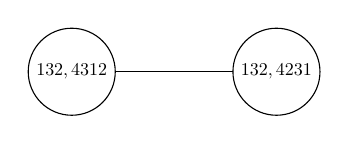
\begin{tikzpicture}[vertex/.style = {shape=circle,draw,minimum size=1.5em},scale=0.65, every node/.style={scale=0.65}]
    \node[vertex] (a) at (0,0) {$\Av{132, 4312}$};
    \node[vertex] (b) at (4,0) {$\Av{132, 4231}$};
    \draw (a) -- (b);
\end{tikzpicture}
%    \caption{The bijection for the first Wilf class of permutations avoiding one pattern of size 3 and one of size 4.}
%    \label{fig:1x31x4bi_1}
%\end{figure}

\begin{figure}[ht!]
    \centering
    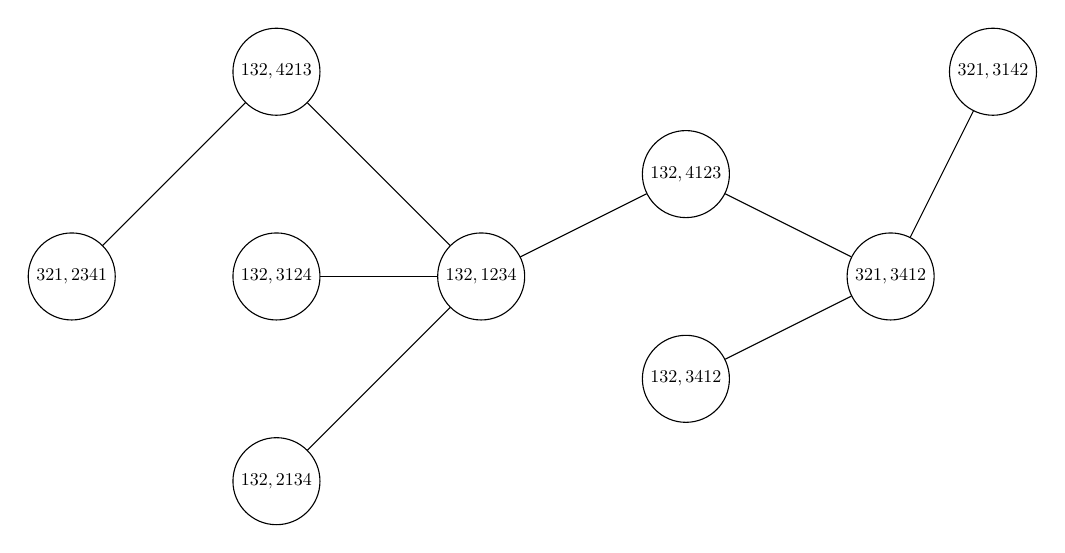
\begin{tikzpicture}[vertex/.style = {shape=circle,draw,minimum size=1.5em},scale=0.65, every node/.style={scale=0.65}]
    \node[vertex] (a) at (-12,0) {$\Av{321, 2341}$};%0-a
    \node[vertex] (b) at (4,0) {$\Av{321, 3412}$};%1-b
    \node[vertex] (c) at (6,4) {$\Av{321, 3142}$};%2-c
    \node[vertex] (d) at (-4,0) {$\Av{132, 1234}$};%3-d
    \node[vertex] (e) at (-8,4) {$\Av{132, 4213}$};%4-e
    \node[vertex] (f) at (0,2) {$\Av{132, 4123}$};%5-f
    \node[vertex] (g) at (-8,0) {$\Av{132, 3124}$};%6-g
    \node[vertex] (h) at (-8,-4) {$\Av{132, 2134}$};%7-h
    \node[vertex] (i) at (0,-2) {$\Av{132, 3412}$};%8-i
    \draw (a) -- (e);
    \draw (d) -- (e);
    \draw (d) -- (f);
    \draw (d) -- (g);
    \draw (d) -- (h);
    \draw (b) -- (f);
    \draw (b) -- (c);
    \draw (b) -- (i);
\end{tikzpicture}
    \caption{The connections created by bijections found for the second Wilf class of permutations avoiding one pattern of size 3 and one of size 4.}
    \label{fig:1x31x4bi_2}
\end{figure}

\subsection{Avoiding one pattern of size 4}
There are two Wilf classes with more than one permutation class. We did not manage to find bijections between $\Av{1342}$ and $\Av{2413}$ which make up one of those Wilf classes. That is because TileScope requires another technique\footnote{The technique is called the \emph{table method} which allows some rules in the universe to be used backwards.} to enumerate them which is not compatible with our bijection searcher. The other consists of $\Av{1234}$, $\Av{1243}$, $\Av{1432}$ and $\Av{2143}$. TileScope lacks the strategies to solve $\Av{2143}$ so that was out of reach while the connections created by bijections found for the others are shown in \FigureRef{fig:1x4bi}.

\begin{figure}[ht!]
    \centering
    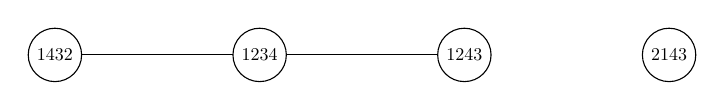
\begin{tikzpicture}[vertex/.style = {shape=circle,draw,minimum size=1.5em},scale=0.65, every node/.style={scale=0.65}]
    \node[vertex] (a) at (0,0) {$\Av{1234}$};
    \node[vertex] (b) at (4,0) {$\Av{1243}$};
    \node[vertex] (c) at (-4,0) {$\Av{1432}$};
    \node[vertex] (d) at (8,0) {$\Av{2143}$};
    \draw (a) -- (b);
    \draw (a) -- (c);
\end{tikzpicture}
    \caption{The connections created by bijections found for the Wilf class of $\Av{1234}$, $\Av{1243}$, $\Av{1432}$ and $\Av{2143}$.}
    \label{fig:1x4bi}
\end{figure}

\subsection{Experimental classes}
The experimental classes we ran our bijection searcher for can be seen in Appendix \ref{ch:expcls}. They are grouped by Roman numerals and figures contain their list indices.

The experiments were carried out by comparing the first class against all others, then the second to all but the first and so on. A disjoint-set data structure was used to keep track of confirmed equivalences. As a consequence, the experiments favored lower numbers to have higher degrees. The setup for the experiments can be seen in Appendix \ref{ch:expsetup}.

Every experimental class was confirmed to be a Wilf class with the exception of experimental class III where we failed to find a bijection between
\[
    \Av{1243,1342,1423,1432,2143,2413,3142,3412,4231}
\]
and any other class. We leave that as an open problem. The connections created by bijections found for each experimental class can be seen in Figures~\ref{fig:expgrp_I}-\ref{fig:expgrp_XXVI} in Appendix \ref{ch:conclusion}. Experimental classes with only two permutation classes are omitted since all of them were successfully shown to be Wilf classes and no information is contained in their figure.